\documentclass[a4paper,12pt]{article}
\usepackage[utf8]{inputenc}
\usepackage[spanish]{babel}
\usepackage{authblk}
\usepackage[left=2.0cm,right=2.0cm,top=2.5cm,bottom=2.5cm]{geometry}

\usepackage{enumerate}
\usepackage{multirow}% http://ctan.org/pkg/multirow
\usepackage{hhline}
\usepackage{longtable}
\usepackage{adjustbox}
\usepackage{bigstrut}
\usepackage{tabulary}
\usepackage{float}
\usepackage{hyperref}

% bibliography

\usepackage[authoryear]{natbib}
\bibliographystyle{abbrvnat}

\usepackage{minted}
% math

\usepackage{amsmath,amsfonts,amssymb}

% images
\usepackage{graphicx} %package to manage images
%\usepackage{subcaption}
\usepackage{subfig}
\usepackage{float}

% para codigo
%\usepackage{minted}
\usepackage{listings}

% \usepackage[noabbrev]{cleveref}
\graphicspath{{/home/laura/Documents/Maestria/2018-1-segundoSemestre/fisica_estadistica_avanzada/ParteII_Johans/Tarea3/parte2/temperatura_fija/}
  {/home/laura/Documents/Maestria/2018-1-segundoSemestre/fisica_estadistica_avanzada/ParteII_Johans/Tarea3/parte2/temperatura_fija_nfijo/}
{/home/laura/Documents/Maestria/2018-1-segundoSemestre/fisica_estadistica_avanzada/ParteII_Johans/Tarea3/parte2/cv_images/} {/home/laura/Documents/Maestria/2018-1-segundoSemestre/fisica_estadistica_avanzada/ParteII_Johans/Tarea3/parte1/images/directo/}}

\title{\textbf{Sistemas de Espínes}}

\author[*]{Laura Catalina Arboleda Hernández}
\affil[*]{Instituto de Física, Universidad de Antioquia}

\renewcommand\Authand{ y }
%\renewcommand\Authands{ y }

%\date{\small{\today}}
\date{}



\begin{document}

 \maketitle


\section{Resumen}

\noindent Se realizó un conteo directo de los microestados de un sistema de $L$ espines para posteriormente estimar la varianza de la energía del sistema y obtener así curvas de calor específico como función de la temperatura. Se encontró que el método de directo es inviable en témrinos computacionales, debido al tiempo de computo al gasto de memoria para almacenar todos los microestados en un sistema real. Además se implementó el modelo de Ising 2D y se usó un método de montecarlo con probabilidad de aceptación de Metropolis para general microestados a partir del cambió de espín de uno de los átomos de la malla del modelo de Ising. Se comprobó que el uso de un muestreo representativo produce resultados muy cercanos a la solución real en sistemas de tamaños de varios tamaños, hasta $64 \times 64$, inalcanzable con el método directo, es decir, que el muestreo reduce el tiempo de computo y la cantidad de memoria requerida. Aún así, el muestreo de monte carlo depende fuertemente del número de pasos o intentos y un número muy grande requiere un tiempo de computo significativo, sobretodo en sistemas mucho más grandes. 

\subsection*{Palabras Clave}

\noindent Modelo de Ising, Monte Carlo, espín, calor específico. 

 \section{Método: Cálculo Directo}

 \noindent Se desarrolló un código en Python para estimar el número de microestados de un sistema $L =  N\times N$ átomos, generándolos todos a partir de una configuración incial dada. El código se muestra a continuación

 \begin{minted}{python}
#-------------------------------------------
# Enegía de cada microestado y energía total 
#-------------------------------------------

def all_microstates_energy(all_microstates,N):

    #tiempo de CPU
    t_init = time.time()

    Etot = E = 0.0
    Ei = []

    for k in range(2**(N*N)):
        
        Emicro = 0.0
       
        micro = all_microstates[k]    
        
        for i in range(N):
            for j in range(N):
            
                #valor de los espín vecinos del átomo [i,j] en el microestado [k] con condiciones de forntera periódicas

                ngb1 = micro[i,(j+1)%N]
                ngb2 = micro[(i-1)%N,j]
                ngb3 = micro[i,(j-1)%N]
                ngb4 = micro[(i+1)%N,j]

                # dividimos entre 2 porque cada interacción se cuenta dos veces
                
                Eij =  micro[i,j]*(ngb1 + ngb2 + ngb3 + ngb4)/2 
                Emicro += Eij
                
        #energía de los microestados individuales
        Ei.append(Emicro)

        #energía total del sistema
        Etot += Emicro
        
    t_end = time.time()
    print("Time: ",t_end-t_init)

    return Ei, Etot


#-------------------------------------
# Generación de todos los microestados 
# Posibles para un sistema de L átomos
# L = N x N
#--------------------------------------

def define_microstates(N):

    L = N*N

    print("Defining microstates...")
    
    #number of configurations
    n_micro = 2**L

    m_prev = [-1]*L

    all_microstates = [np.reshape(np.array(m_prev),(N,N))]
    
    for i in range(n_micro-1):
    
        k = 0
    
        m = m_prev[:]
    
        while m[k] == 1:
        
            m[k] = -1
        
            k = k + 1
        
        m[k] = 1
    
        m_prev = m[:]
            
        all_microstates.append(np.reshape(np.array(m),(N,N)))
        
    return(all_microstates)


#----------------------------
#Programa Principal
#----------------------------

if len(sys.argv) < 2:
    N = 4
else:
    N = int(sys.argv[1])

print("Running with %d x %d"%(N,N))

all_microstates = define_microstates(N)

Ei, Etot = all_microstates_energy(all_microstates,N)


#--------------------------
# histograma de texto
#--------------------------

energias, OmegaE = np.unique(Ei,return_counts = True)
for i in range(len(energias)):
    print(energias[i],"\t",OmegaE[i])

#--------------------------------------------
# Histograma de energias de los microestados
#--------------------------------------------

n_bins = 100

plt.hist(Ei, bins = n_bins)


   \end{minted}

   \noindent Con este código se generaron los microestados correspondientes a sistemas $2 \times 2$, $3 \times 3$ y $4 \times 4$. Dado que el costo computacional es muy alto, pues el número de microestados es $2^L$, en la realidad es impráctico usar el método directo y en este caso no se pudo simular sistemas mayores $4 \times 4$. Los resultados se muestran en la figura \ref{fig:histogramas-directo}. Se observa que el histograma para $3 \times 3$ no es simétrico, lo cuál se debe a que es un número impar de átomo por lo que la malla en la que se disponen no es cuadrada, sino rectángular. En la figura \ref{fig:histograma-texto} se muestra la densidad de estados, es decir, el número de estados que tienen un valor dado de energía. 

   \begin{figure}[H]
     \centering
     \subfloat[]{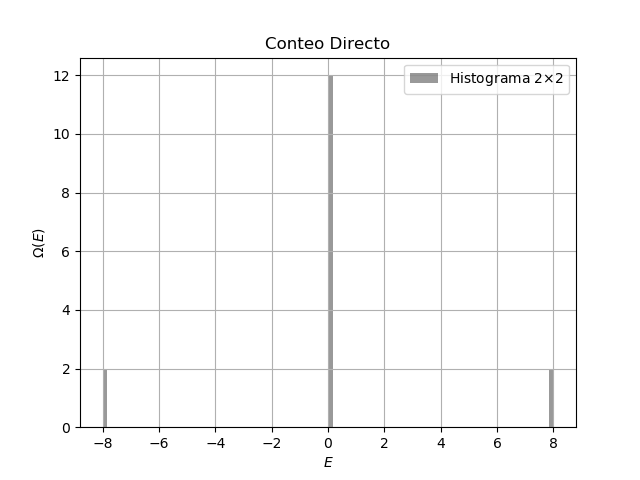
\includegraphics[width=6.0cm]{histograma_2x2}}
     \subfloat[]{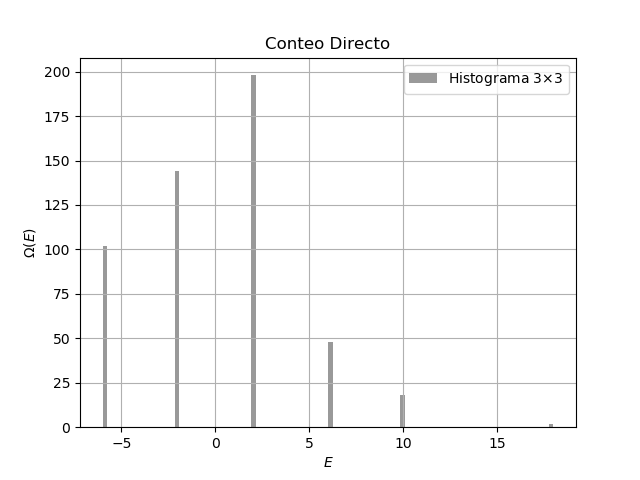
\includegraphics[width=6.0cm]{histograma_3x3}}
     \subfloat[]{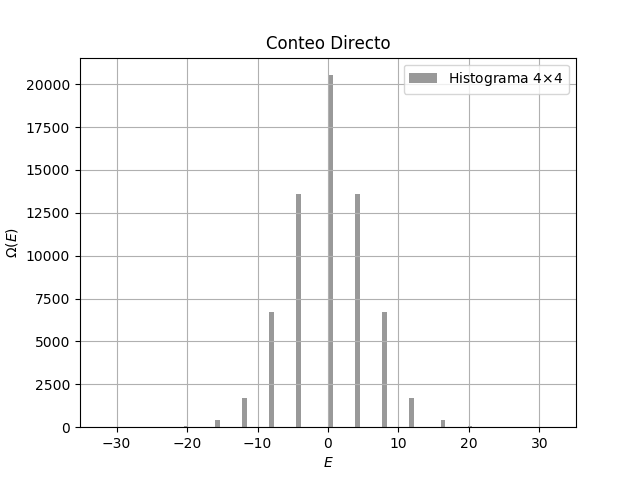
\includegraphics[width=6.0cm]{histograma_4x4}}
     \caption{Histogramas de energías para sitemas de tamaño: (a)  $2 \times 2$, (b) $3 \times 3$ y (c) $4 \times 4$}
     \label{fig:histogramas-directo}
   \end{figure}

     \begin{figure}[H]
     \centering
     \subfloat[]{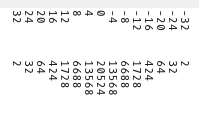
\includegraphics[width=6.0cm]{histo_texto_4x4}}
     \caption{Densidad de estados para el sistema $4 \times 4$.}
     \label{fig:histograma-texto}
   \end{figure}

   \subsection{Calor Específico}

\noindent El calor específico representa el incremento en la energía internal del sistema causado por un aumento \textit{infinitesimal} en la temperatura, es decir

\begin{equation}
C_{v} = \frac{\partial \langle E \rangle}{\partial T} =  \frac{\partial \beta}{\partial T} \frac{\partial \langle E \rangle}{\partial \beta}
\end{equation}

\noindent En unidades naturales, $\beta = 1/T$, luego $\partial \beta / \partial T = -1/T^2 = -\beta^2$. Con esto, el calor específico por partícula se puede escribir como

\begin{align}
  c_{V}= \frac{C_{V}}{N} &= -\frac{\beta ^2}{N}\frac{\partial \langle E \rangle}{\partial \beta}\nonumber \\
                         &= -\frac{\beta ^2}{N} \frac{\partial}{\partial \beta}\left[ \frac{1}{\mathcal{Z}} \sum_{r} E_{r} e^{-\beta E_{r}} \right]\nonumber \\
                         &= -\frac{\beta ^2}{N} \left[ \frac{\partial}{\partial \beta} \left( \frac{1}{\mathcal{Z}}\right)\sum_{r} E_{r} e^{-\beta E_{r}} +  \frac{1}{\mathcal{Z}} \frac{\partial}{\partial \beta} \left( \sum_{r} E_{r} e^{-\beta E_{r}}\right) \right]\nonumber \\
                         &=  -\frac{\beta ^2}{N} \left[ -\frac{1}{\mathcal{Z}^2} \frac{\partial \mathcal{Z}}{\partial \beta} \sum_{r} E_{r} e^{-\beta E_{r}} -  \frac{1}{\mathcal{Z}}  \sum_{r} E_{r}^2 e^{-\beta E_{r}}  \right]
                           \label{eq:cv}
\end{align}

\noindent La función partición está dada por

\begin{equation}
\mathcal{Z} = \sum_{r} e^{-\beta E_{r}} \Longrightarrow  \frac{\partial \mathcal{Z}}{\partial \beta} = -\sum_{r} E_{r}e^{-\beta E_{r}}
  \end{equation}

  \noindent Así, la ecuación en \ref{eq:cv} se reescribe como

  \begin{align}
    c_{V}  &= \frac{\beta ^2}{N} \left[ -\frac{1}{\mathcal{Z}^2}\left( \sum_{r} E_{r} e^{-\beta E_{r}}\right)^2 +  \frac{1}{\mathcal{Z}}  \sum_{r} E_{r}^2 e^{-\beta E_{r}}  \right]
             \label{eq:cv1}
\end{align}

\noindent Además, se tiene que

\begin{equation}
  \langle E \rangle = \frac{1}{\mathcal{Z}} \sum_{r} E_{r} e^{-\beta E_{r}}
  \label{eq:valormedioE}
\end{equation}

\begin{equation}
  \langle E^2 \rangle = \frac{1}{\mathcal{Z}} \sum_{r} E_{r}^2 e^{-\beta E_{r}}
  \label{eq:valormedioE2}
  \end{equation}

  \noindent Reemplazando \ref{eq:valormedioE} y \ref{eq:valormedioE2} en la ecuación \ref{eq:cv1}, el calor específico por partícula es entonces

  \begin{equation}
    \frac{\beta ^2}{N} \left( \langle E^2 \rangle - \langle E \rangle ^2 \right)
    \label{eq:cvfinal}
  \end{equation}
  
  
   \section{Modelo de Ising}

   \noindent Se realizó un algorítmo para la implementación del modelo de Ising en 2D. Este modelo describe la interación entre los espines de un conjunto de átomos que se configuran en una malla, en este caso 2D, con condiciones de forntera periódicas. Cada átomo puede tener un espín $+1$ ó $-1$ y las interacciones con sus primeros vecinos (espines en la malla) pueden provocar un cambio de espín. Los vecinos de un punto en la malla (átomo) se definen como se muestra en la figura \ref{fig:vecinos}

    \begin{figure}[H]
     \centering
     \subfloat[]{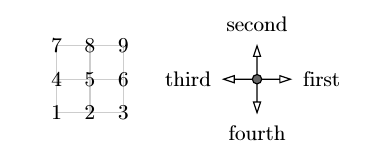
\includegraphics[width=9.0cm]{vecinos}}
     \caption{Esquema de primeros vecinos para el modelo de Ising 2D. Tomado de \cite{krauth2006}.}
     \label{fig:vecinos}
   \end{figure}

   \noindent La energía está dada por

   \begin{equation}
     E = -J\sum_{\langle k,l \rangle}\sigma_{k} \sigma_{l}
   \end{equation}
   \noindent En donde $\sigma_{k} \pm 1$, con $k = 1,...,N$ los átomos en la malla. La suma es sobre todos los pares de vecinos, pero considerando una sola vez la interacción entre un par, es decir ya sea la interacción $\langle k, l \rangle$ ó $\langle l,k \rangle$. Se desarrolló un código en python que usa una técnica de monte carlo para realizar un muestreo representativo sobre un microestado inicial, considerando posibilidad de cambio de espín de uno de los átomos en la malla, con probabilidad de aceptación de Metropolis. De esta forma, al aceptar un cambió de espín se genera un nuevo microestado. La idea es estimar la energía del sistema sin tener que considerar el número total de microestados ($\Omega = 2^L, L = N \times N$), sino sólo una cantidad representativa, que suponemos exhibira bien las propiedades del sistema. 
   
   \begin{minted}{python}
     
#---------------------------------------------------------
# Función para generar un estado de la malla aleatorio:
# cada átomo en un estado de espín aleatorio
#---------------------------------------------------------

def initial_microstate(N):   
    #microestado aleatorio de L átomos. L = N x N
    state = 2*np.random.randint(2, size=(N,N))-1
    return state

#---------------------------------------------------------
# Movidas de monte carlos usando el algoritmo Metropolis 
# para generar o no un microestado nuevo
#---------------------------------------------------------

def monte_carlo_realization(microstate, N, beta):
   
    for i in range(N):
        for j in range(N):
            
            #escogemos aleatoriamente la posición del 
            #átomo (s) en la malla: (fila(a),columna(b))
                
            a = np.random.randint(0, N) #0 y N-1
            b = np.random.randint(0, N)
            
            s =  microstate[a, b]
                
            #vecinos del átomo s:
            ngb1 = microstate[a,(b+1)%N]
            ngb2 = microstate[(a-1)%(N),b]
            ngb3 = microstate[a,(b-1)%N]
            ngb4 = microstate[(a+1)%(N),b]
            
            deltaE = 2*s*(ngb1 + ngb2 + ngb3 + ngb4)
            
            if deltaE < 0: #acepte con probabilidad igual 1 el cambio de espín
                s *= -1
            elif random.uniform(0.0,1.0) < np.exp(-deltaE*beta):
                s *= -1
                    
            #cambie el espín del átomo y guardelo en su posición, 
            #esto genera un nuevo microestado
            microstate[a, b] = s
                
    return microstate

#----------------------------
# Energía de un microestado
#----------------------------

def microstate_energy(microstate, N):
    energy = 0
    for i in range(len(microstate)):
        for j in range(len(microstate)):
            #S: espín del átomo en la fila i columna j
            S = microstate[i,j]
            ngb1 = microstate[i,(j+1)%N]
            ngb2 = microstate[(i-1)%N, j]
            ngb3 = microstate[i,(j-1)%N]
            ngb4 = microstate[(i+1)%N, j]
            energy += -S*(ngb1 + ngb2 + ngb3 + ngb4)/2     
    return energy

#---------------------------------
# Magnetización de un microestado
#---------------------------------

def magnetization(microstate):
    mag = np.sum(microstate)
    return mag

#--------------------------------
# parámetros para las pruebas
#--------------------------------

#------------------------------
#tamaño de la malla: L = N x N
#------------------------------

N = [6,32,128]      

#-------------------------------------
# Temperatura fija
#-------------------------------------

T = [0.1,1.0,2.269,5.0]

#---------------------
#pasos de monte carlo
#---------------------

n_steps = 10000

for k in N:

    #--------------------------------------------
    #fijar configuración inicial para una T fija
    #--------------------------------------------
    
    Microstate = initial_microstate(k)

    for j in T:

         E = []
         M = []
         t_steps = []
         E_cumulative = []
         E_cum = 0.0

         beta = 1/j
        
         for i in range(n_steps):
        
            monte_carlo_realization(Microstate, k, beta)
        
            #energía
            Ene = microstate_energy(Microstate, k)
        
            #magnetización
            Mag = magnetization(Microstate) 
            
            #guardamos solo los valores del muestreo 
            #respresentativo correspondientes 
            #a la relajación del sistema: equilibrio
             
            if i>(n_steps/3):
                t_steps.append(i)
                E.append(Ene)
                M.append(Mag)
                E_cum =  E_cum + Ene
                E_cumulative.append(E_cum/(i+1))

         Emean = sum(E)/len(E)       
         print("Energía media \t = %f"%Emean)
                
         #-----------------        
         #archivo de datos
         #-----------------
                
         f = open('datos_tfix_nfix/%dx%d_T%0.1f_nsteps%d.dat'%(k,k,j,n_steps),'w')
        
         for p in range (len(E)):
             f.write("%d %.8f %d %.8f\n"%(t_steps[p], E[p], M[p], E_cumulative[p]))
         f.close()
        
         #-----------------------
         #graficas snap final
         #-----------------------

         plt.imshow(Microstate)
      
         #-----------------------
         #graficas E vs t_steps
         #-----------------------
         
         plt.plot(t_steps,E)
        
         #--------------------------
         #graficas E_cum vs t_steps
         #--------------------------

         plt.plot(t_steps,E_cumulative)
        
       \end{minted}

   \subsection{Temperatura Fija}

   \noindent Se realizó la prueba del código para una temperatura fija y varios tamaños del arreglo de espines. En la figura \ref{fig:snaps_6x6} se muestra la configuración final dada por el muestreo de monte carlo para distinto número de pasos (o variaciones del microestado inicial) para un sistema de 36 espines ($N = 6$) a $T = 2.0 K$.
   \noindent En la tabla \ref{tab:e_per_spin} se concluye que al aumentar el número de pasos de montecarlo, el resultado se acerca más al valor obtenido con enumeración exacta y la energía media por espín se acerca más al valor $\langle E \rangle /L = -1.7473$.

   \begin{table}[H]
     \begin{center}
       \begin{tabular}{| l | c |}
         \hline
         n      & $\langle E \rangle/L$  \\ \hline
         100    & -1.73737375    \\ \hline
         1000   & -1.72856188889 \\
         10000  & -1.74627463889 \\ \hline
         100000 & -1.74591913889 \\
         \hline
       \end{tabular}
       \caption{Valores de energía media por espín para el sistema $6 \times 6$ ($L = 36$), variando el número de pasos de monte carlo ($n$).}
       \label{tab:e_per_spin}
     \end{center}
\end{table}

% 6x6, T=2.0
\begin{figure}[H]
  \centering
  \subfloat[]{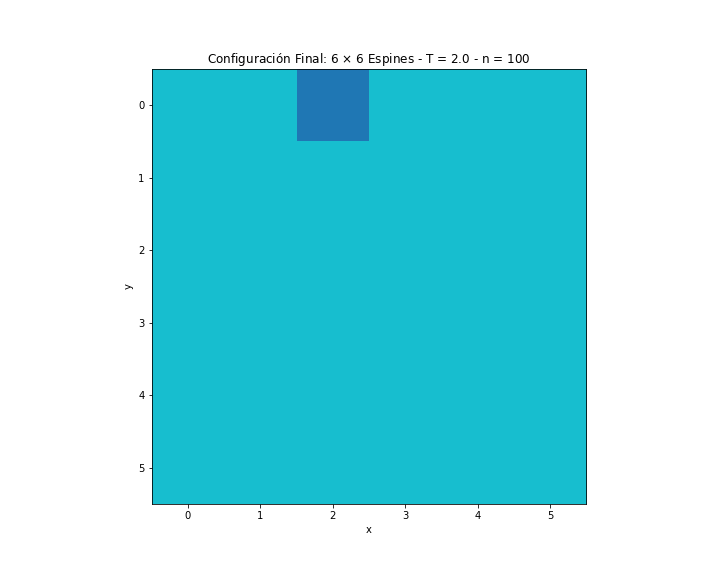
\includegraphics[width=9.0cm]{finalsnap_6x6_T2_steps100}}
  \subfloat[]{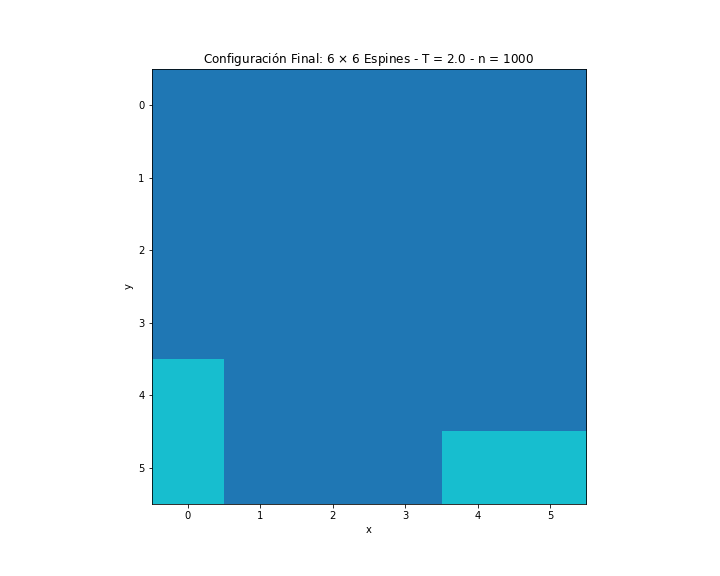
\includegraphics[width=9.0cm]{finalsnap_6x6_T2_steps1000}}\\
  \subfloat[]{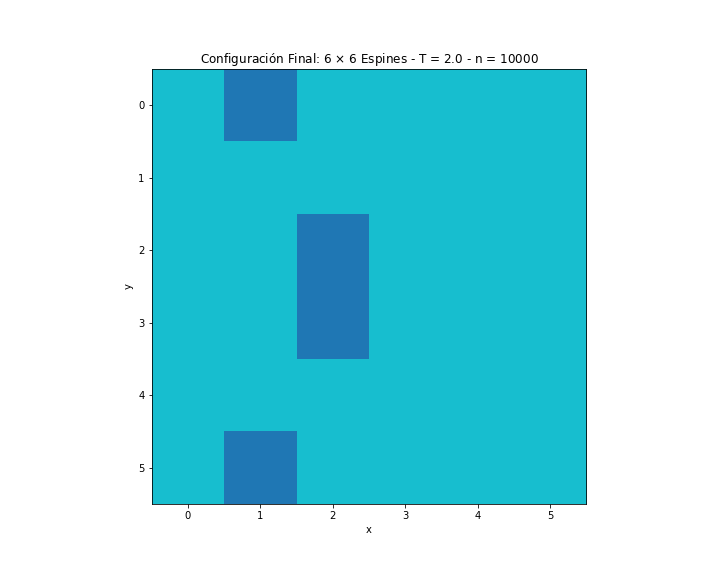
\includegraphics[width=9.0cm]{finalsnap_6x6_T2_steps10000}}
  \subfloat[]{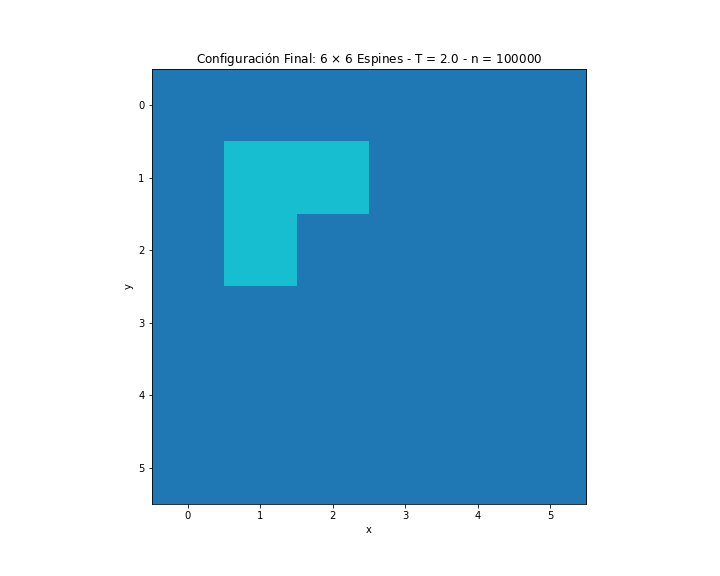
\includegraphics[width=9.0cm]{finalsnap_6x6_T2_steps100000}}
  \caption{Configuración final típica para un sistema de $6 \times 6$ átomos para $T = 2.0 K$ diferente número de pasos de montecarlo.}
  \label{fig:snaps_6x6}
\end{figure}


\noindent Se dejó fijo el número de pasos de monte carlo en $n = 10000$ y se varió la temperatura para el sistema $128 \times 128$ y $32 \times 32$ pasando por la temperatura crítica, en donde el sistema pasa del régimen ferromagnético al paramagnético. Los resultados se muestran en las figuras \ref{fig:snaps_32x32} y \ref{fig:snaps_128x128}. Se observa que a bajar temperaturas ($T = 0.1 K$) el sistema está dominado ya sea por átomos con espín arriba o por átomos con espín abajo. A medida que aumenta la temperatura ($T = 5.0 K$) se puede observar que la configuración espín arriba o espín abajo, ambas, son igualmente probables, luego, la cantidad de puntos azul claro y oscuro es aproximadamente la misma.


% 32x32
\begin{figure}[H]
  \centering
  \subfloat[]{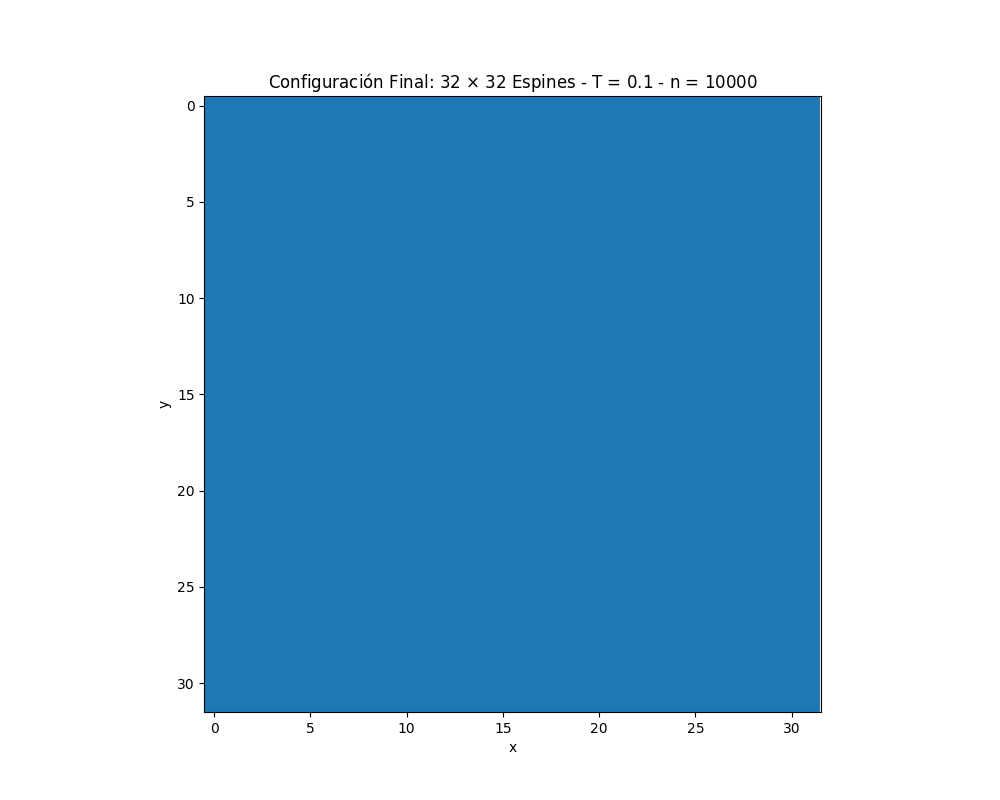
\includegraphics[width=9.0cm]{finalsnap_32x32_T0_nsteps10000}}
  \subfloat[]{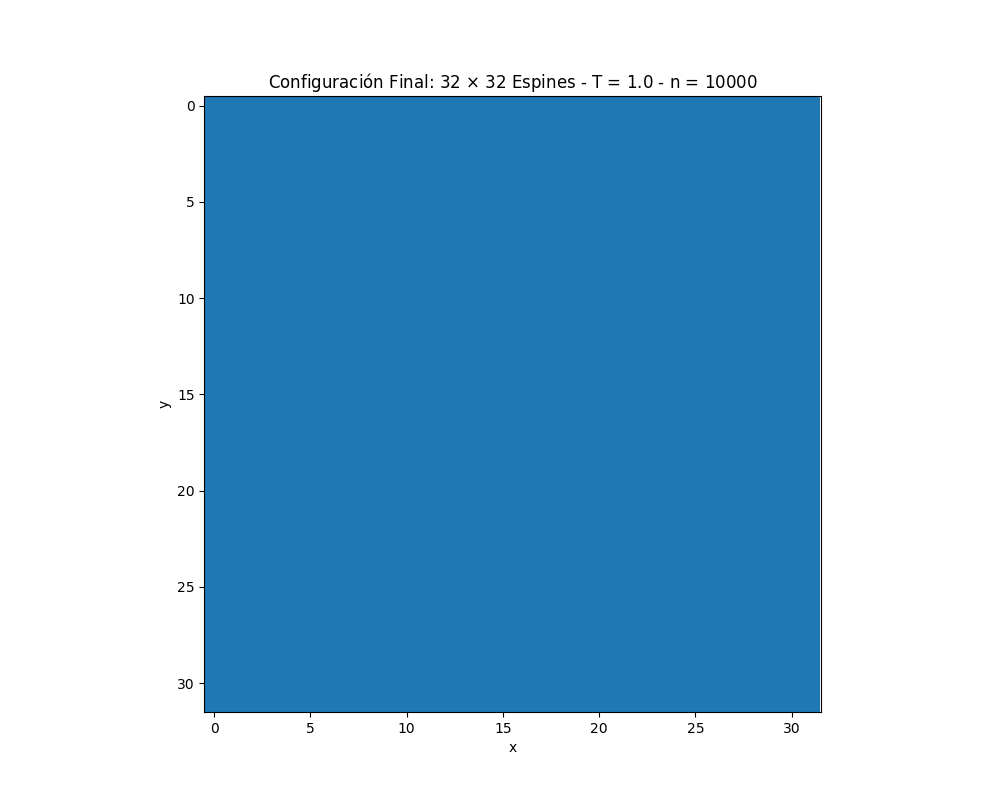
\includegraphics[width=9.0cm]{finalsnap_32x32_T1_nsteps10000}}\\
  \subfloat[]{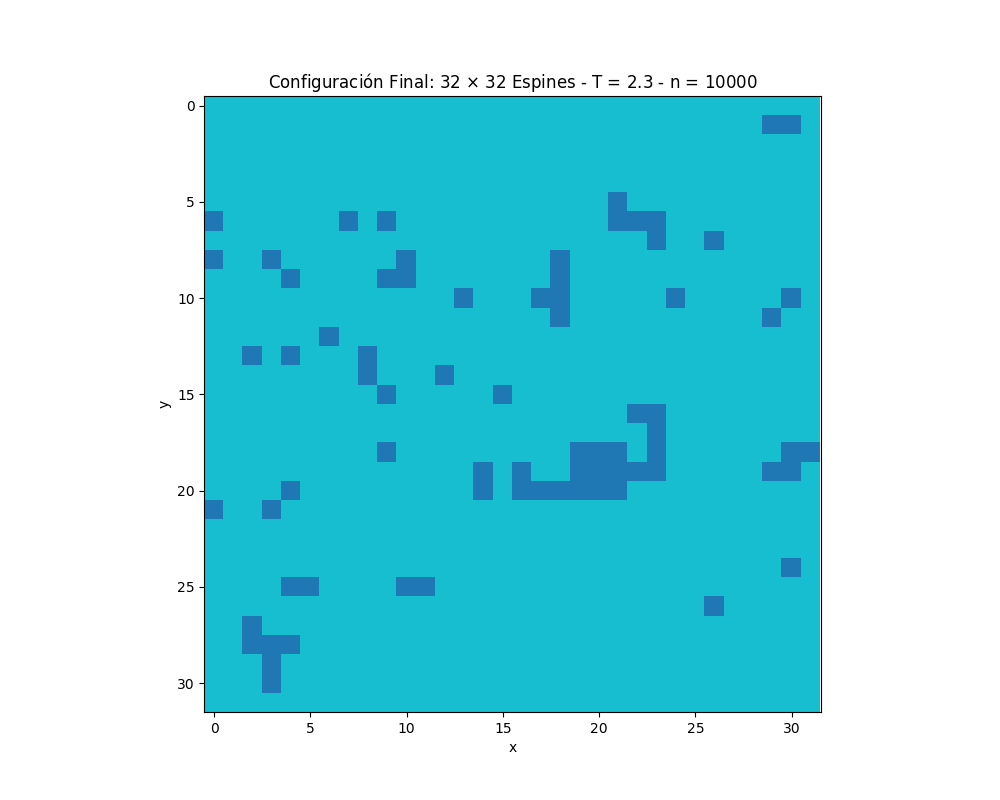
\includegraphics[width=9.0cm]{finalsnap_32x32_T2_nsteps10000}}
  \subfloat[]{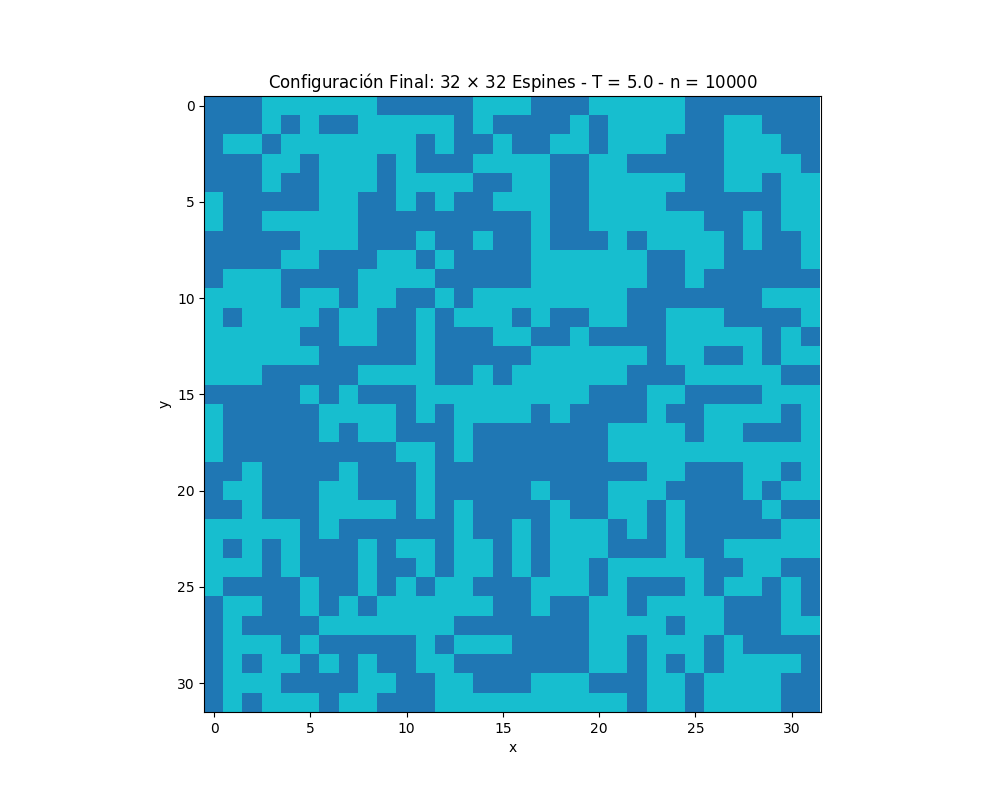
\includegraphics[width=9.0cm]{finalsnap_32x32_T5_nsteps10000}}     
  \caption{Configuración final típica para un sistema de $32 \times 32$  átomos para distintas temperaturas y $n = 10000$ pasos de montecarlo.}
  \label{fig:snaps_32x32}
\end{figure}

% 128x128
\begin{figure}[H]
  \centering
  \subfloat[]{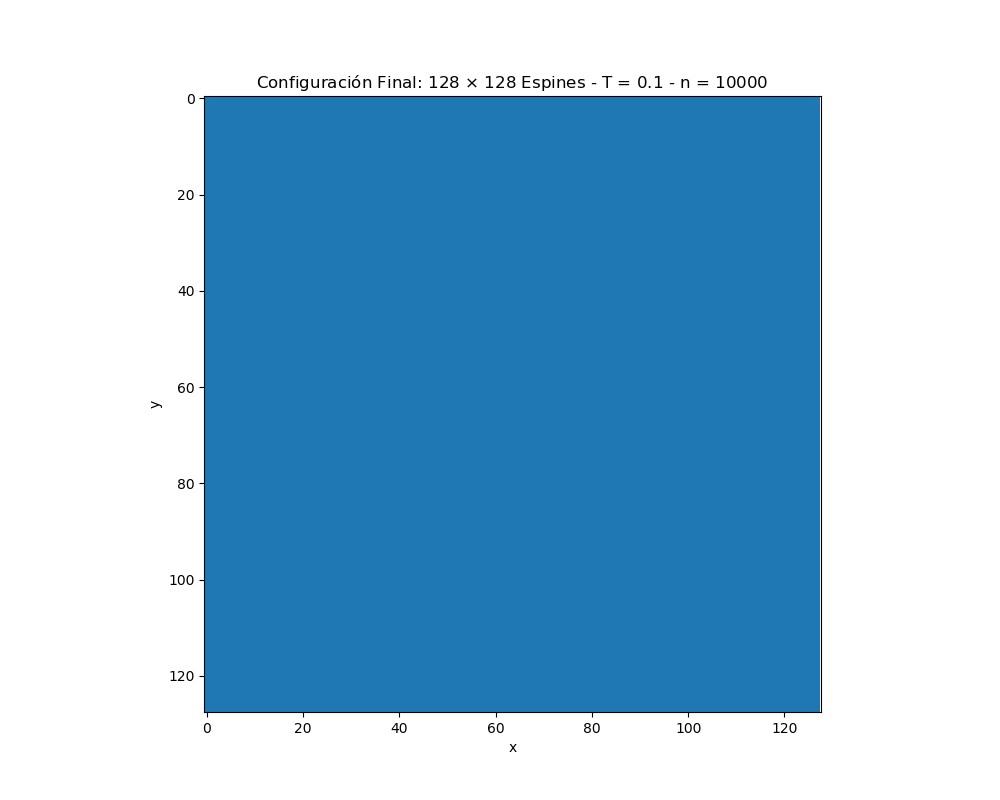
\includegraphics[width=9.0cm]{finalsnap_128x128_T0_nsteps10000}}
  \subfloat[]{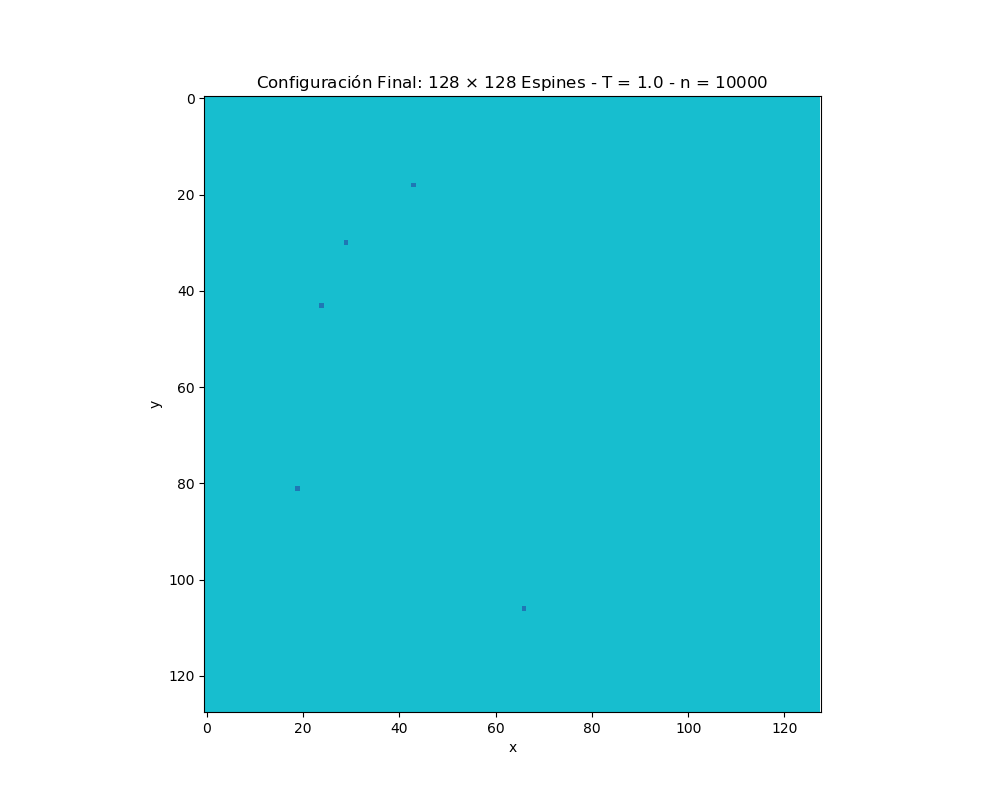
\includegraphics[width=9.0cm]{finalsnap_128x128_T1_nsteps10000}}\\
  \subfloat[]{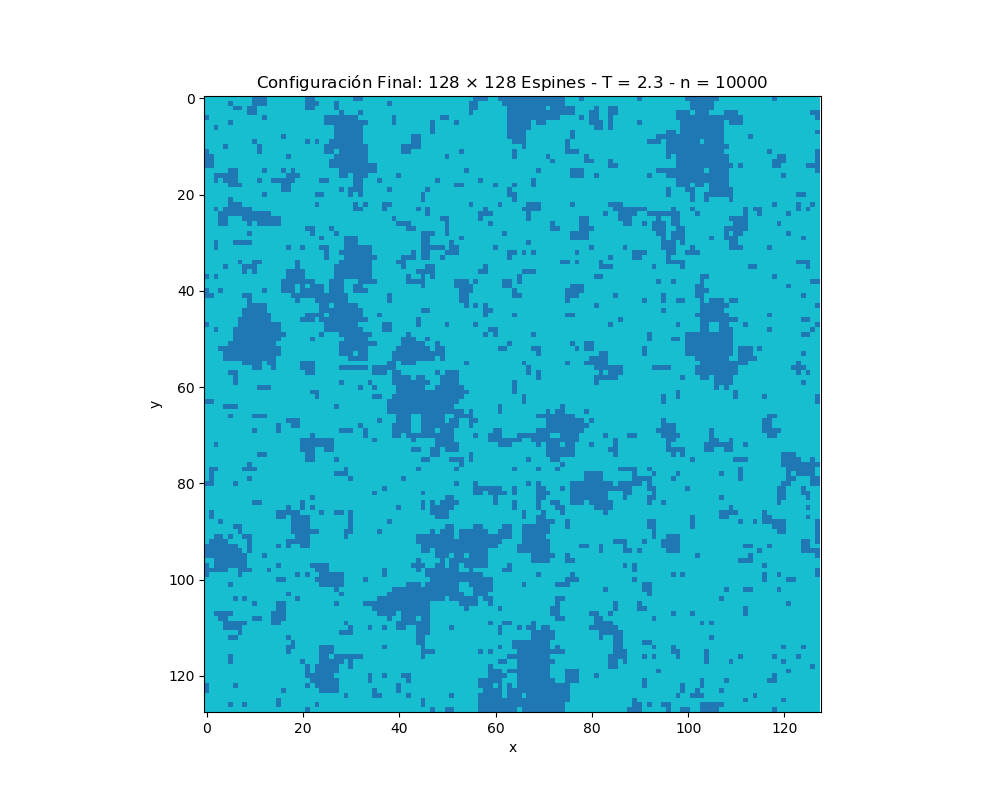
\includegraphics[width=9.0cm]{finalsnap_128x128_T2_nsteps10000}}
  \subfloat[]{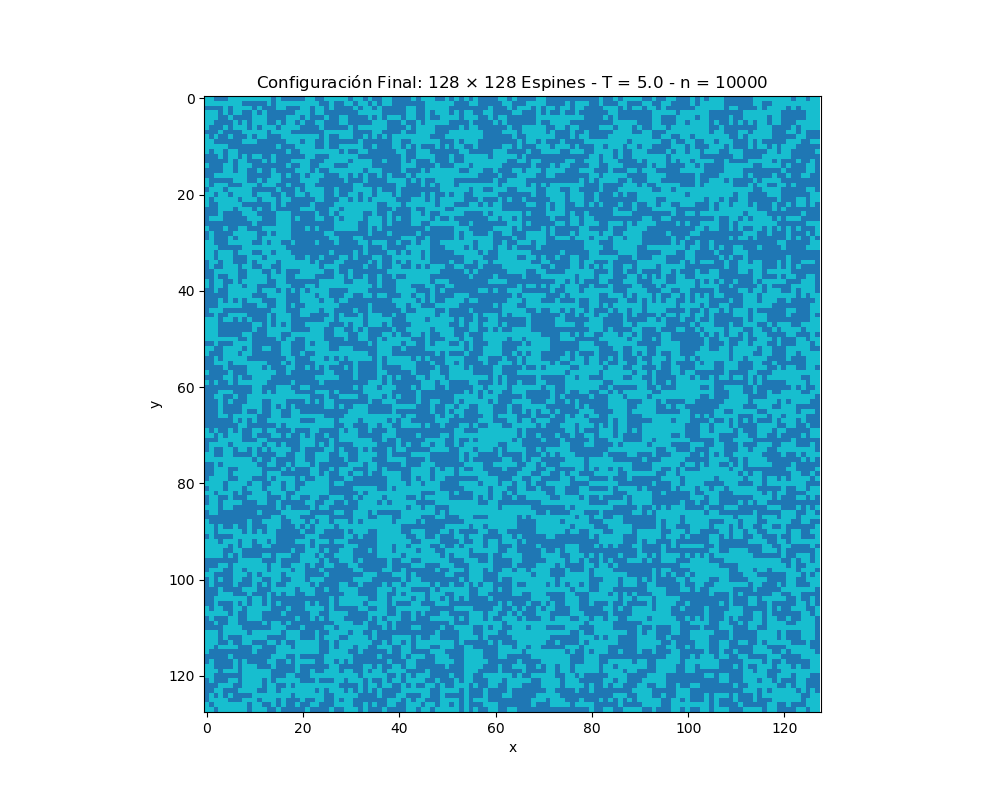
\includegraphics[width=9.0cm]{finalsnap_128x128_T5_nsteps10000}}     
  \caption{Configuración final típica para un sistema de $128 \times 128$ átomos para distintas temperaturas y $n = 10000$ pasos de montecarlo.}
  \label{fig:snaps_128x128}
\end{figure}

\noindent Se graficó la energía en cada configuración muestreada con monte carlo (metropolis) y la energía acumulada en cada paso del muestreo para el sistema  $128 \times 128$ a $T = T_{c} \approx 2.3$
\begin{figure}[H]
  \centering
  \subfloat[]{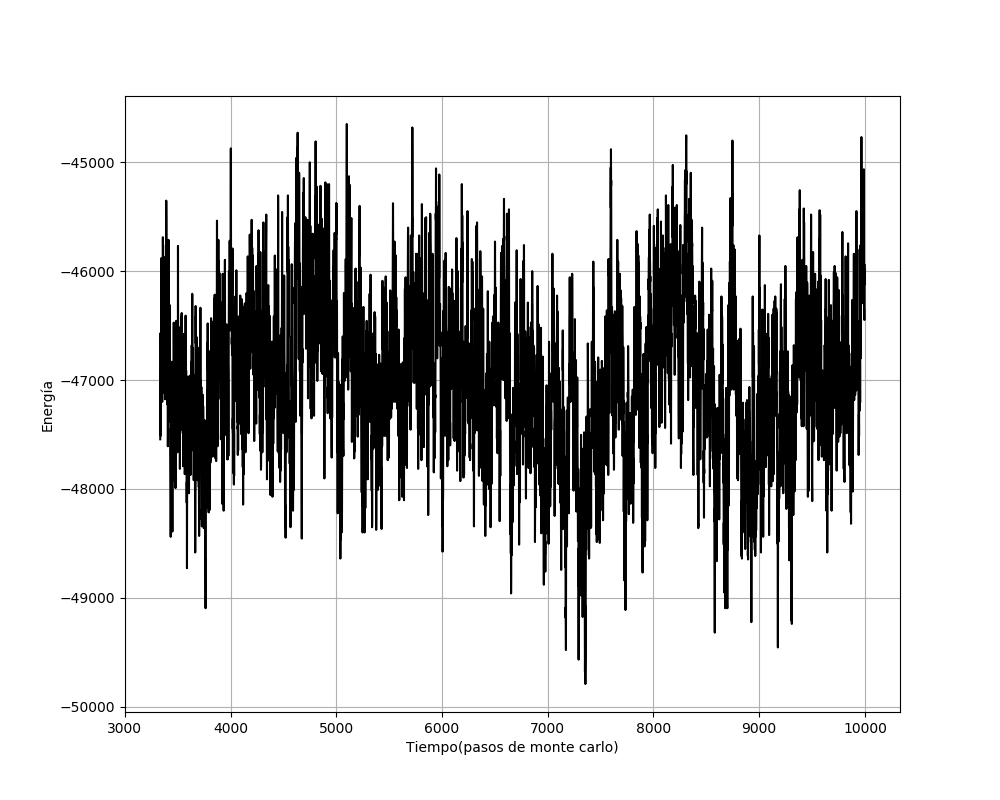
\includegraphics[width=9.0cm]{E_time_128x128_T2_nsteps10000}}
  \subfloat[]{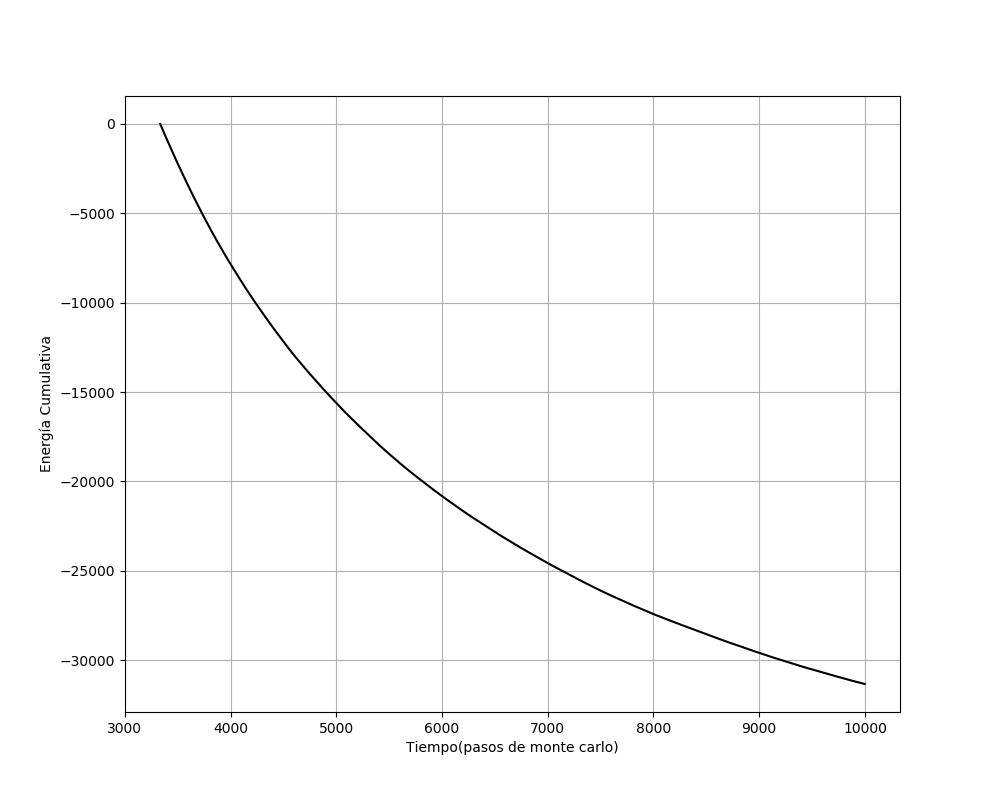
\includegraphics[width=9.0cm]{Ecum_time_128x128_T2_nsteps10000}}
  \caption{Sistema de $128 \times 128$ átomos a $T_{c} = 2.269 K$. (a) Energía de los microestados muestreados con $10000$ pasos de montecarlo (b) Energía cumulativa de los microestados para los mismos $10000$ pasos.}
  \label{fig:E_time_128x128}
\end{figure}


\subsection{Energía Media y Calor Específico}

\noindent Con base en el teorema de fluctuación-disipación se realizaron muestreos de montecarlo para diferentes valores de temperatura, y se estimó el valor medio de la energía para cada temperatura como

\begin{equation}
  \langle E \rangle = \sum_{i=1}^{S} E_{i}
\end{equation}


\noindent Donde $E_{i}$ es el valor de energía de una configuración del sistema de espines dada con el muestreo de montecarlo. El índice $i$ representa un paso de montecarlo y $S$ indica que sólo sumaremos los M pasos que corresponden al sistema ya en equilibrio, es decir, la cantidad de puntos del muestreo representativo, es decir, no todas la configuraciones generadas representan el sistema en el equilibrio, solo después de un tiempo suficientemente largo (un número alto de pasos de monte carlo), el sistema estará en un estado de relajación y cada configuración representará a el sistema en un estado de equilibrio. Para un sistema ferromagnético, la energía de una configuración dada es

\begin{equation}
  E_{i} = \sum_{<k,l>} \sigma_{k} \sigma_{l}
\end{equation}

\noindent El valor esperado de la magnetización se obtuvousando el mismo principio del muestreo representativo como

\begin{equation}
  \langle M \rangle = \sum_{i=1}^{S} M_{i}
\end{equation}

\noindent En este caso la magnetización de una configuración o microestado dado por un paso de monte carlo es

\begin{equation}
  M_{i} = \sum_{i} \sigma_{i}
\end{equation}

\noindent Se usó el mismo código descrito en la sección anterior para el muestreo de monte carlo con probabilidad de aceptación de Metropolis, pero esta vez estimando la magnetización y la energía media, como se muestra a continuación

\begin{minted}{python}
         
#------------------------------
#tamaño de la malla: L = N x N
#------------------------------

N = [2,4,8,16,64]      

#-------------------------------------
# Temperatura fija
#-------------------------------------

Tc = 2.269
Betac = 0.4407

n_steps = 4000

T =np.arange(0.05,4,0.1)

nt = np.size(T)

n_bins = 100

E_mean         = np.zeros(nt)
E2_mean        = np.zeros(nt)
Magnetization  = np.zeros(nt)
SpecificHeat   = np.zeros(nt)

SpecificHeat_arr = []
plt.figure(figsize=(10,8))
for j in N:
    
    Microstate = initial_microstate(j)
    
    for k in range(len(T)):

        E = []
        M = []
        all_E = []
    
        beta=1.0/T[k]; beta2=beta**2

        for i in range(n_steps):

        
            monte_carlo_realization(Microstate,j, beta)
        
            #energía
            Ene = microstate_energy(Microstate,j)
        
            #magnetización
            Mag = magnetization(Microstate) 

            all_E.append(Ene)
            
            if i>(n_steps/3):
                E.append(Ene)
                M.append(Mag)
                
        E_mean[k]            = sum(E)/len(E)
        E2_mean[k]           = sum(p**2 for p in E)/len(E)
        SpecificHeat[k]      = (beta2/j)*(E2_mean[k] - (E_mean[k]**2)) 
        Magnetization[k]     = sum(M)/len(M)
        
           
    SpecificHeat_arr.append(SpecificHeat.copy())

    #------------------------
    #graficas individuales
    #------------------------
    
    #energía vs T    

    plt.plot(T, E_mean)
   
    #magnetización vs T

    plt.plot(T, abs(Magnetization))
    
 
#grafica calor específico: todos los tamaños

for j in range(len(N)):
    plt.plot(T, SpecificHeat_arr[j], '-', label=r"%d $\times$ %d"%(N[j],N[j]))

  \end{minted}
       
       \noindent La figura

       \begin{figure}[H]
         \centering
         \subfloat[]{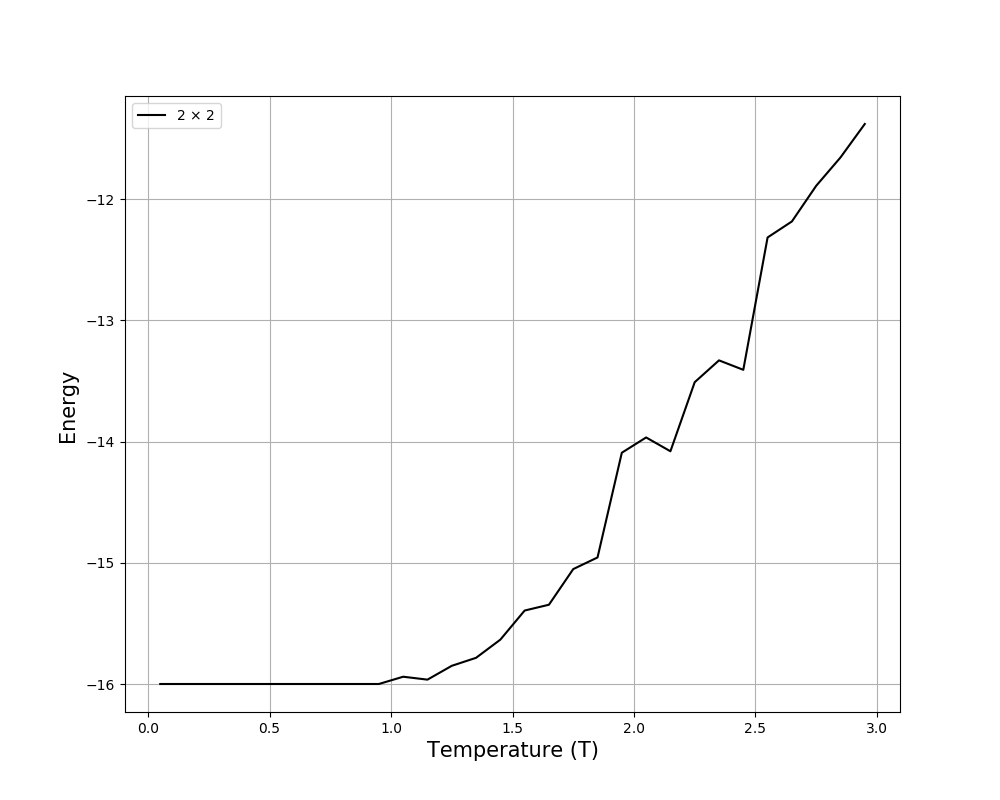
\includegraphics[width=8.0cm]{2x2energia}}
         \subfloat[]{\label{fig:2x2magnetization}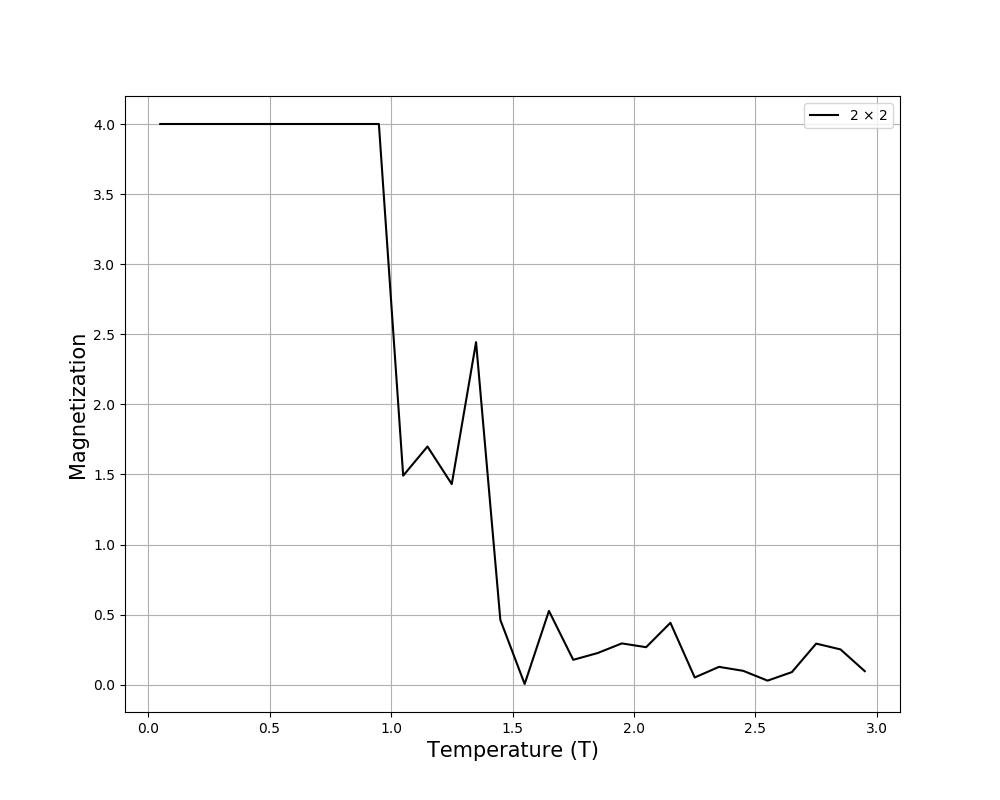
\includegraphics[width=8.0cm]{2x2magnetizacion}}\\
         \subfloat[]{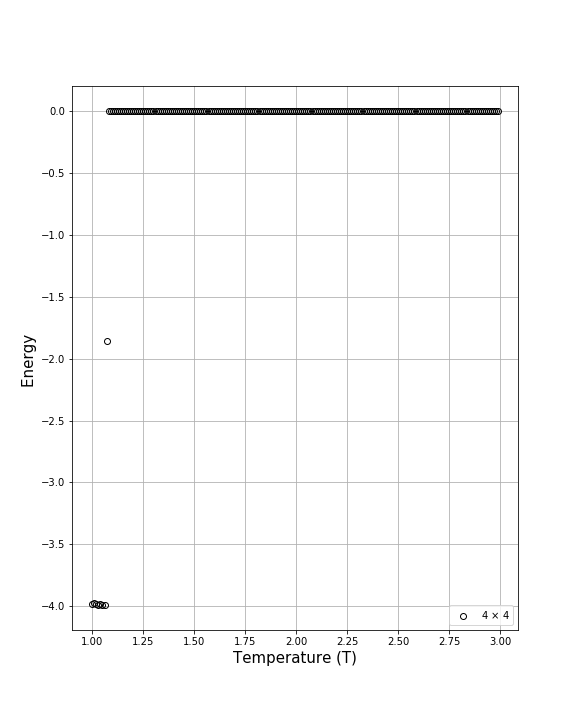
\includegraphics[width=8.0cm]{4x4energia}}
         \subfloat[]{\label{fig:4x4magnetization}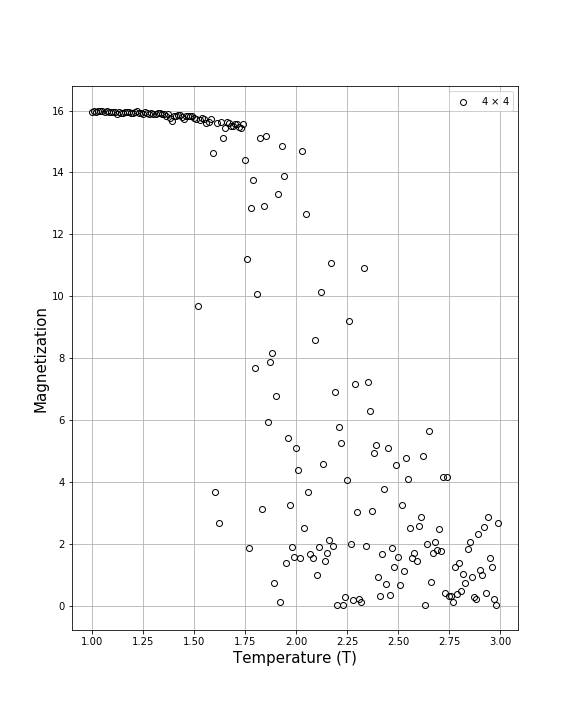
\includegraphics[width=8.0cm]{4x4magnetizacion}}
          \caption{Valor esperado de la energía y la magnetización para un sistema de espines (a) $2 \times 2$ y (b) $4 \times 4$ con 5000 pasos de monte carlo.}
         \label{fig:EM1}
       \end{figure}

       
       \begin{figure}[H]
         \centering
         \subfloat[]{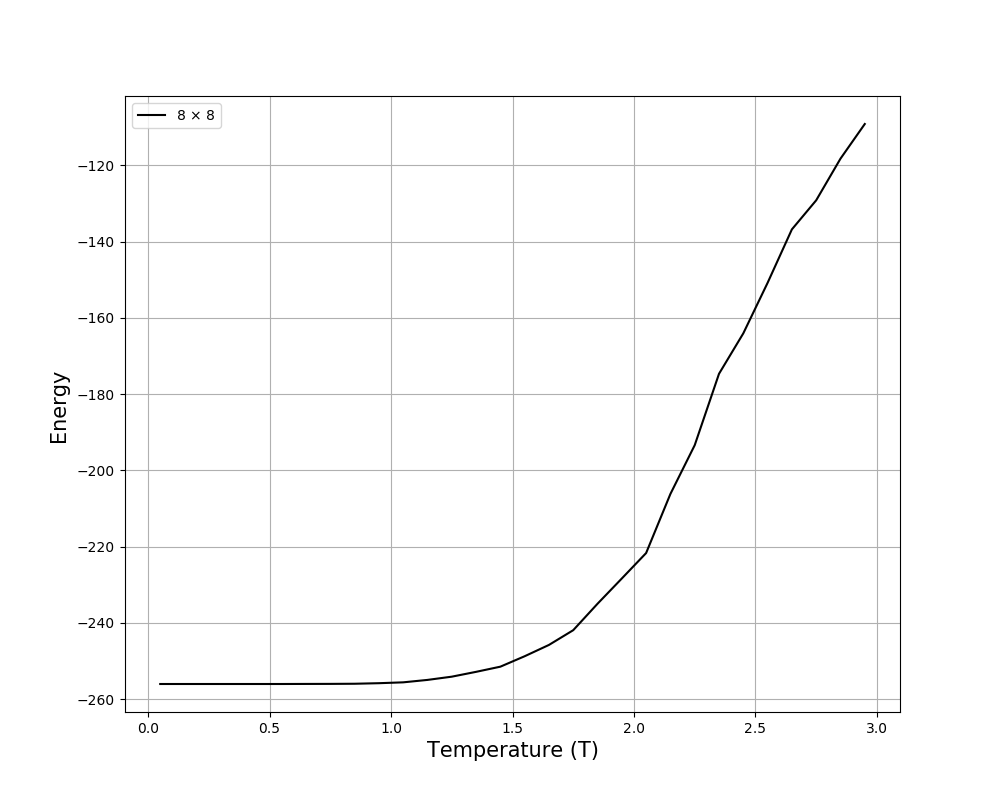
\includegraphics[width=8.0cm]{8x8energia}}
         \subfloat[]{\label{fig:8x8magnetization}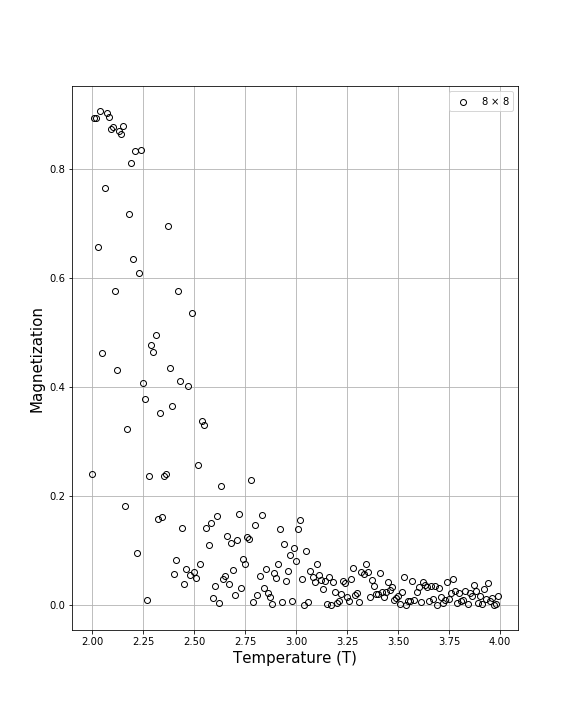
\includegraphics[width=8.0cm]{8x8magnetizacion}}\\
         \subfloat[]{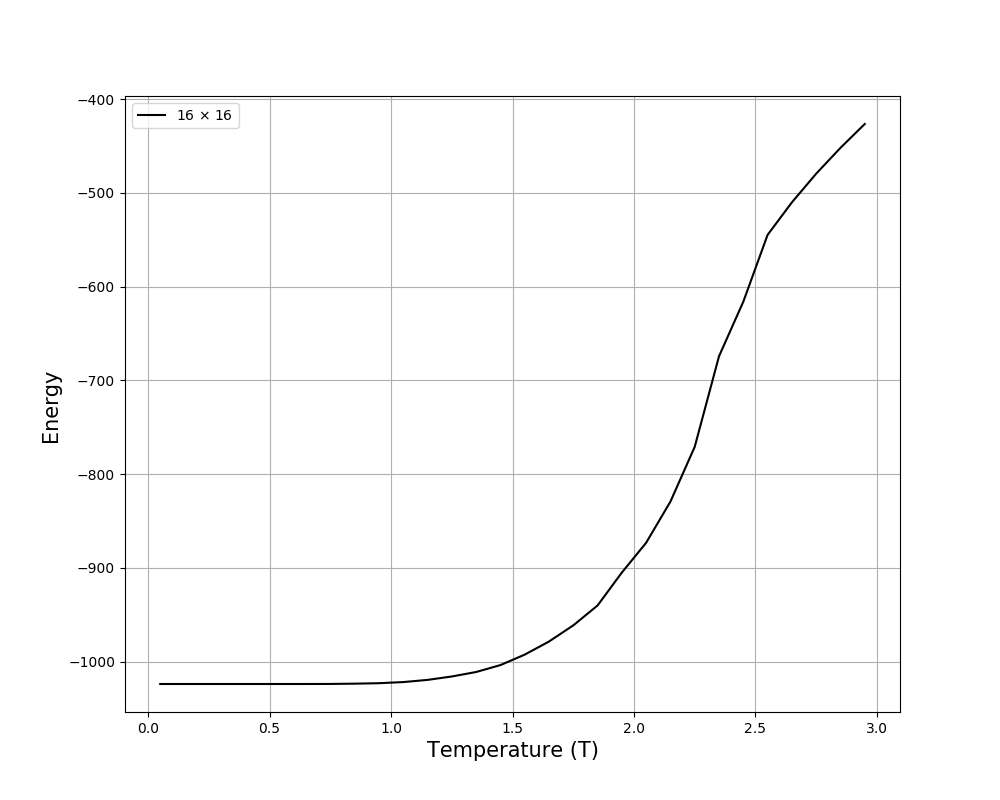
\includegraphics[width=8.0cm]{16x16energia}}
         \subfloat[]{\label{fig:16x16magnetization}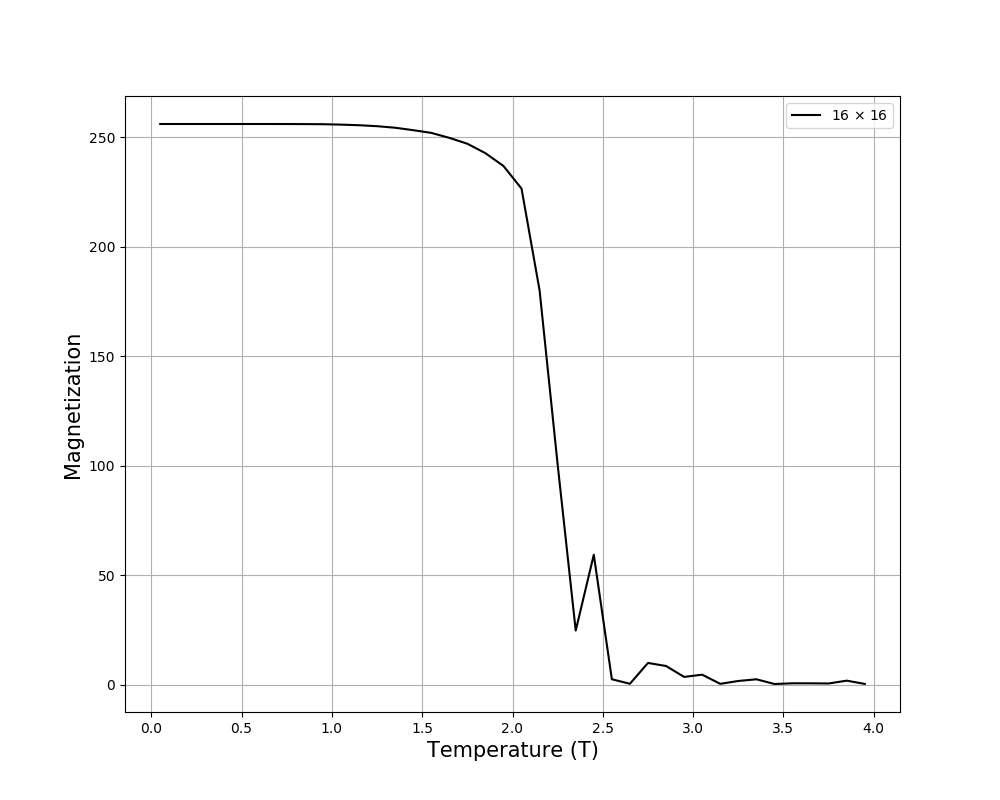
\includegraphics[width=8.0cm]{16x16magnetizacion}}
         \caption{Valor esperado de la energía y la magnetización para un sistema de espines (a) $8 \times 8$ y (b) $16 \times 16$ con 5000 pasos de monte carlo.}
         \label{fig:EM2}
       \end{figure}

       
       \noindent En la figura \ref{fig:cv} se muestran las curvas de calor específica para sistemas de espines de diferente tamaño. Se observa que el calor específico decae a cero a medida que la temperatura se acerca al cero absoluto. Así, se comprueba la tercera ley de la termodinámica,  el cero absoluto es inalcanzable. Por otro lado, se puede observar que el pico del calor específico (máximo) se corre hacia la izquierda a medida que el tamaño de la distribución aumenta. El calor específico diverge en $T = T_{c} = 2.269$. Por encima de esta temperatura, a temperaturas altas, el sistema es paramagnético, lo que puede observarse por ejemplo en la figura \label{fig:16x16magnetization} en donde vemos que por encima de $T_{c}$ la magnetización es cero. Por debajo de $T_{c}$ el sistema es ferromagnético.
       
        \begin{figure}[H]
         \centering
         \subfloat[]{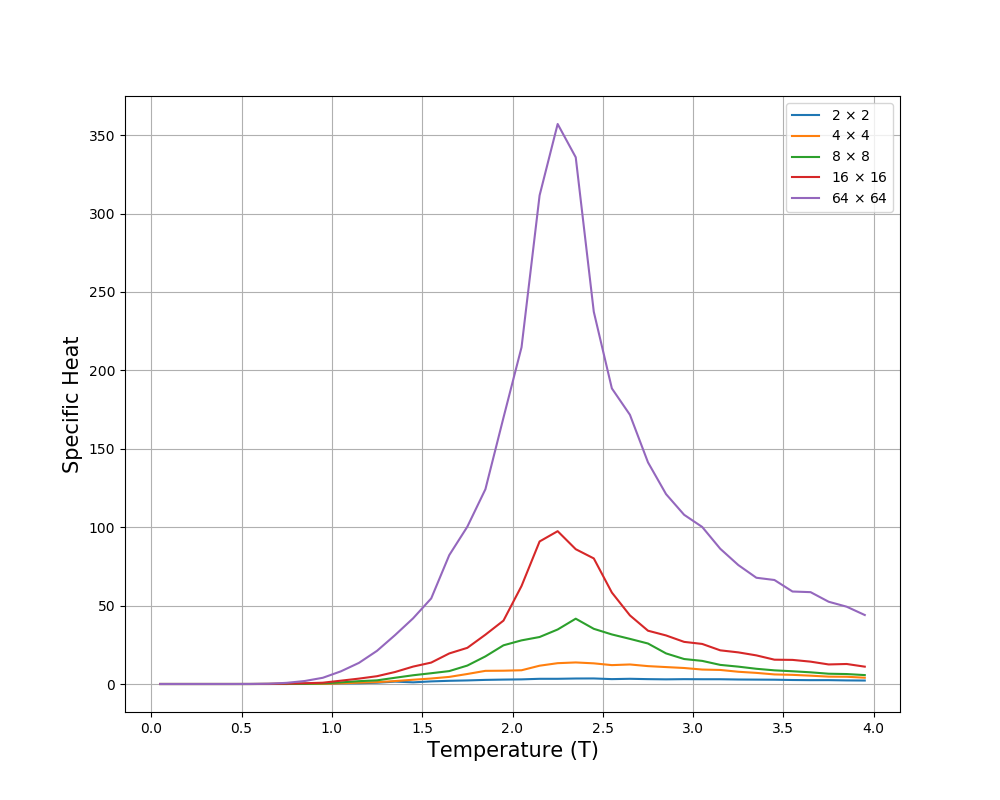
\includegraphics[width=9.0cm]{cv_todos}}
         \caption{Curvas de calor específico para sistemas de espines de diferente tamaño.}
         \label{fig:cv}
       \end{figure}

       
   \noindent 

   
   
 % \section{Bibliografía}
\bibliography{informe}


\end{document}


%%% Local Variables:
%%% TeX-command-extra-options: "-shell-escape"
%%% mode: latex
%%% TeX-master: t
%%% End: